\documentclass[physicsII_notes.tex]{subfiles}
\begin{document}
\section{Aula 21 - 09/10/2023}
\subsection{Motivações}
\begin{itemize}
	\item Ondas;
	\item Classificação das Ondas;
	\item A Equação da Onda.
\end{itemize}
\subsection{Ondas e Classificações}
As ondas fazem transporte de energia e momento. Exemplos delas incluem o som, terremotos,
ondas d'água e a própria luz, possuindo aplicações em diversas áreas do cotidiano. Estudaremos
esse fenômeno, desde suas classificações à sua descrição físico-matemática.

Começando pelas classificações, existem dois tipos principais de ondas - as transversais e as longitudinais.
A melhor forma de pensar nas transversais é pensando que elas têm um formato de, enquanto que as longitudinais
aparentam ser um monte de barra vertical que juntam-se e separam-se. Como exemplo
das ondas transversais, vide o gráfico abaixo:

\begin{center}
	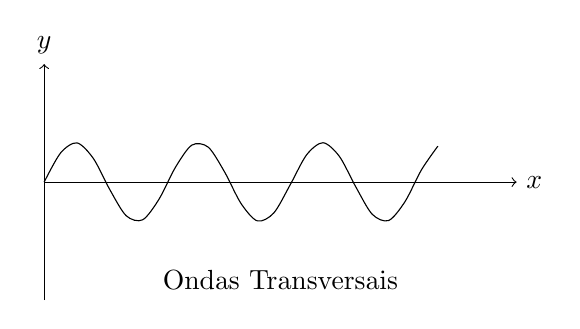
\begin{tikzpicture}
		\draw[->] (0,0) -- (6,0) node[right] {$x$};
		\draw[->] (0,-1.5) -- (0,1.5) node[above] {$y$};
		\draw[scale=0.5,domain=0:10,smooth,variable=\y,shift={(0,0)}]
		plot ({\y},{sin(2*\y r)});
		\node[below] at (3,-1.0) {Ondas Transversais};
	\end{tikzpicture}
\end{center}

e, para as longitudinais, a seguir está o exemplo:

\begin{center}
	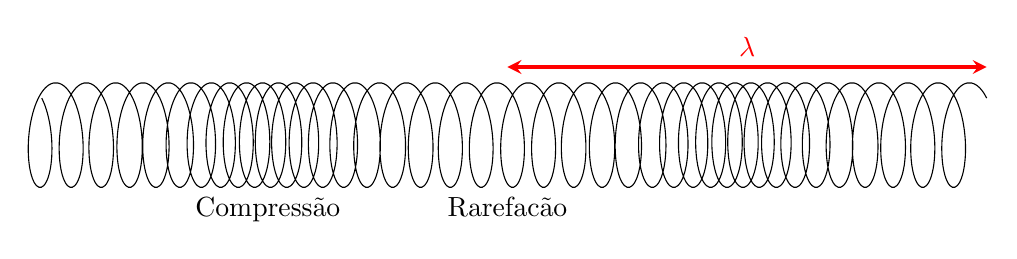
\begin{tikzpicture}
		\begin{scope}[z={(70:1)},y={(110:1)},local bounding box=coil]
			\draw plot[domain=0:14400,variable=\t,samples=1441,smooth]
			({\t/1200+0.1*pi*sin(\t/20)},{-0.5*sin(\t)},{0.5*cos(\t)});
		\end{scope}
		\path (coil.south west) -- (coil.south east)
		node[pos=0.25,below]{Compressão} node[pos=0.5,below]{Rarefacão};
		\draw[very thick,red,stealth-stealth]
		([yshift=2mm]coil.north) -- ([yshift=2mm]coil.north east)
		node[midway,above]{$\lambda$};
	\end{tikzpicture}
\end{center}

\subsection{A Equação da Onda - Primeiros Passos}
Ao analisarmos o gráfico de uma onda, vemos que a posição dela no momento t é dada por
\[
	x = vt + x'.
\]
Desta forma, \(x' = x - vt\), o que permite-nos escrever uma forma para a função de propagação dela. Quando
é da esquerda para a direita - ou seja, + x - \(f(x') = f(x-vt)\) e, da direita pra esquerda, -x, é \(f(x') = f(x+vt)\).
Nosso próximo passo é continuar essa análise a fim de encontrar uma equação que descreverá as ondas, começando pelo exemplo
mais simples da corda.

Para que uma corda vibre, ela precisa estar tensionada com tensão \(F_{T}\). Suponha, também, que ela possui densidade de massa \(\mu\).
Passados t segundos, ela é deformada tal qual passa a parecer uma rampa inclinada. O pedaço que ela estava tem tamanho
\(v\Delta t\), enquanto que a altura será \(u\Delta t\), sendo u a velocidade com que ela subiu e v a velocidade da onda.
Para que ela fosse levantada, uma forçá vertical \(F_{y}\) foi exercida. Junto da tração de antes, a soma dessas duas resulta em uma
força \(\vec{F} = \vec{F}_{y} + \vec{F}_{T}.\) De forma mais analítica,

\underline{\textbf{Analisando o Sistema em y:}}

A equação de momento linear no eixo y será
\[
	F_{y}\Delta t = \Delta p = \Delta mu.
\]

Dividindo as duas forças presentes, segue que
\[
	\frac{F_{y}}{F_{t}} = \frac{\Delta tu}{\Delta tv} = \frac{u}{v}.
\]
Assim, juntando as duas equações, segue que
\[
	\frac{\Delta m u}{\Delta t F_{t}} = \frac{u}{v},
\]
ou seja,
\[
	\frac{\Delta m}{\Delta t F_{t}} = \frac{1}{v}.
\]
Utilizando aproximações \(\Delta m\approx \mu v\Delta t,\) chegamos em
\[
	\frac{\mu v\Delta t}{\Delta t F_{t}} = \frac{1}{v} \Rightarrow v^{2}=\frac{F_{t}}{\mu} \Rightarrow v = \sqrt[]{\frac{F_{T}}{\mu}}.
\]
\begin{example}
	Considere uma corda presa à ponta de um telhado e, amarrado a ela, há um peso de \(m=10kg\). Esta corda
	tem comprimento L de 25m e ela sofre uma perturbação na ponta, gerando um pulso a \(20m \) do começo dela. Além disso,
	nesse começo, tem uma lagarta, a \(\Delta x = 2.5cm\) da ponta da corda e movendo-se com \(v'=2.5cm/s\). A massa da
	lagarta é de \(1kg\). Quanto tempo leva para o pulso chegar à lagarta?

	A velocidade do pulso é dada por
	\[
		v = \sqrt[]{\frac{F_{T}}{\mu}}=\sqrt[]{\frac{M_{g}}{\frac{m}{L}}} = \sqrt[]{\frac{10\times 10\times 25}{1}}=50m/s.
	\]
	Com isso, somos capazes de descobrir o tempo que leva para o pulso alcançar a lagarta como
	\[
		\Delta t = \frac{l}{v} = \frac{20}{50} = 0.4s.
	\]
	O tempo para a lagarta atingir em segurança a borda seria
	\[
		\Delta t' = \frac{\Delta x}{v'} = 1s.
	\]
\end{example}
\subsection{Velocidade do Som}
Supondo um gás ideal, no qual PV = NkT, vale que
\[
	v = \sqrt[]{\frac{B}{\rho }},
\]
em que \(B = \frac{-\Delta P}{\frac{\Delta V}{V}}.\) Assim,
\[
	v = \sqrt[]{\frac{\gamma RT}{M}},
\]
e, já que \(\gamma \) e R são constantes, essa velocidade só depende da massa e da temperatura do fluído no qual
o som percorrerá.
\subsection{Deduzindo a Equação da Onda}
Voltando à situação da corda, pegue um pedacinho dela com comprimento \(\Delta x\) e altura \(\Delta y\). Além disso,
na sua extremidade mais alta, uma força \(\vec{F}_{2}\) faz ângulo \(\theta_{2}\) com o eixo horizontal. Analogamente,
na extremidade mais baixa, uma força \(\vec{F}_{1}\) faz ângulo \(\theta_{1}\) com a reta horizontal. Suponha que
\(\theta_{1}, \theta_{2} << 1\), tal que \(\Delta m = \mu\Delta x.\) Vejamos os movimentos em cada eixo.

\underline{\textbf{Eixo x:}}

Como não há movimento em x, a somatória das forças nesse eixo deve ser nula:
\[
	\sum\limits_{}^{}F_{x} = 0 \Rightarrow F_{2}\cos^{}{(\theta_{2})} - F_{1}\cos^{}{(\theta_{1})} = 0.
\]
Como os ângulos são muito pequenos, \(\cos^{}{(\theta_{i})} = 1,  i=1, 2\), ou seja,
\[
	F_{1} = F_{2} \Rightarrow F_{1} = F_{2} = F_{T}.
\]

\underline{\textbf{Eixo y:}}

Aqui, há movimento, de onde vale a segunda Lei de Newton
\[
	\sum\limits_{}^{}F_{y} = \Delta m \frac{\partial^{2}y}{\partial t^{2}}.
\]
Do raciocínio inicial, sabemos que
\begin{align*}
	 & y_{+} = y(x-vt), \\
	 & y_{-} = y(x+vt).
\end{align*}

Unindo com a parte de x, obtemos a equação
\[
	F_{T}\sin^{}{(\theta_{2})} - F_{T}\sin^{}{(\theta_{1})} = \Delta m \frac{\partial^{2}{y}}{\partial{t^{2}}}
\]
Como o ângulo é muito pequeno, \(\sin^{}{(\theta )} = \tan^{}{(\theta )}\). Assim, colocando
\begin{align*}
	 & s_{2} = \tan^{}{(\theta_{2})} = \frac{\partial^{}y}{\partial x^{}}\biggl|_{2}^{}\biggr.  \\
	 & s_{1} = \tan^{}{(\theta_{1})} = \frac{\partial^{}y}{\partial x^{}}\biggl|_{1}^{}\biggr.,
\end{align*}
a equação torna-se
\[
	F_{T}(s_{2}-s_{1}) = \Delta x\mu \frac{\partial^{2}y}{\partial t^{2}}.
\]
Logo,
\begin{align*}
	            & F_{T}\frac{\Delta S}{\Delta x} = \mu \frac{\partial^{2}y}{\partial t^{2}}                                              \\
	\Rightarrow & \lim_{\Delta x\to 0}\frac{\Delta S}{\Delta x}= \frac{\partial^{}S}{\partial x^{}}=\frac{\partial^{2}y}{\partial x^{2}} \\
	\Rightarrow & F_{T}\frac{\partial^{2}y}{\partial x^{2}}=\mu \frac{\partial^{2}y}{\partial t^{2}}                                     \\
	\Rightarrow & \frac{\partial^{2}y}{\partial x^{2}}=\frac{\mu}{F_{T}}\frac{\partial^{2}y}{\partial t^{2}}.
\end{align*}
Portanto, a equação da onda na corda é a seguinte:
\[
	\boxed{\frac{\partial^{2}y}{\partial x^{2}}=\frac{\mu}{F_{T}}\frac{\partial^{2}y}{\partial t^{2}}}
\]

Apesar de termos derivado isso para uma corda, ela vale para todos os tipos de ondas. De fato, para
\(y = y(x-vt)\) qualquer, coloque \(\alpha  = x - vt\). Então,
\begin{align*}
	            & \frac{\partial^{}y}{\partial x^{}} = \frac{\partial^{}y}{\partial \alpha ^{}}\frac{\partial^{}\alpha }{\partial x^{}} = \frac{\partial^{}y}{\partial \alpha ^{}} \\
	\Rightarrow & \frac{\partial^{2}y}{\partial x^{2}} = \frac{\partial^{2}y}{\partial \alpha ^{2}}                                                                                \\
	            & \frac{\partial^{}y}{\partial t^{}}=\frac{\partial^{}y}{\partial \alpha ^{}}\frac{\partial^{}\alpha }{\partial t^{}}=\frac{\partial^{}y}{\partial x^{}}(-v)       \\
	\Rightarrow & \frac{\partial^{2}y}{\partial t^{2}}=v^{2}\frac{\partial^{2}y}{\partial \alpha ^{2}}.
\end{align*}
Juntando ambas, obtemos
\begin{align*}
	            & \frac{1}{v^{2}}\frac{\partial^{2}y}{\partial t^{2}}=\frac{\partial^{2}y}{\partial x^{2}}  \\
	\Rightarrow & \frac{\partial^{2}y}{\partial x^{2}}=\frac{1}{v^{2}}\frac{\partial^{2}y}{\partial t^{2}}.
\end{align*}
Portanto, a equação da onda em sua forma geral é dada por
\[
	\hypertarget{wave_eqn}{\boxed{\frac{\partial^{2}y}{\partial x^{2}}=\frac{1}{v^{2}}\frac{\partial^{2}y}{\partial t^{2}}}}
\]
\end{document}
